% Author: Giulio Stramondo, Mail: giuliostramondo[at]gmail.com
\documentclass{standalone}
\usepackage{tikz}
\usetikzlibrary{positioning,arrows,patterns}
\begin{document}
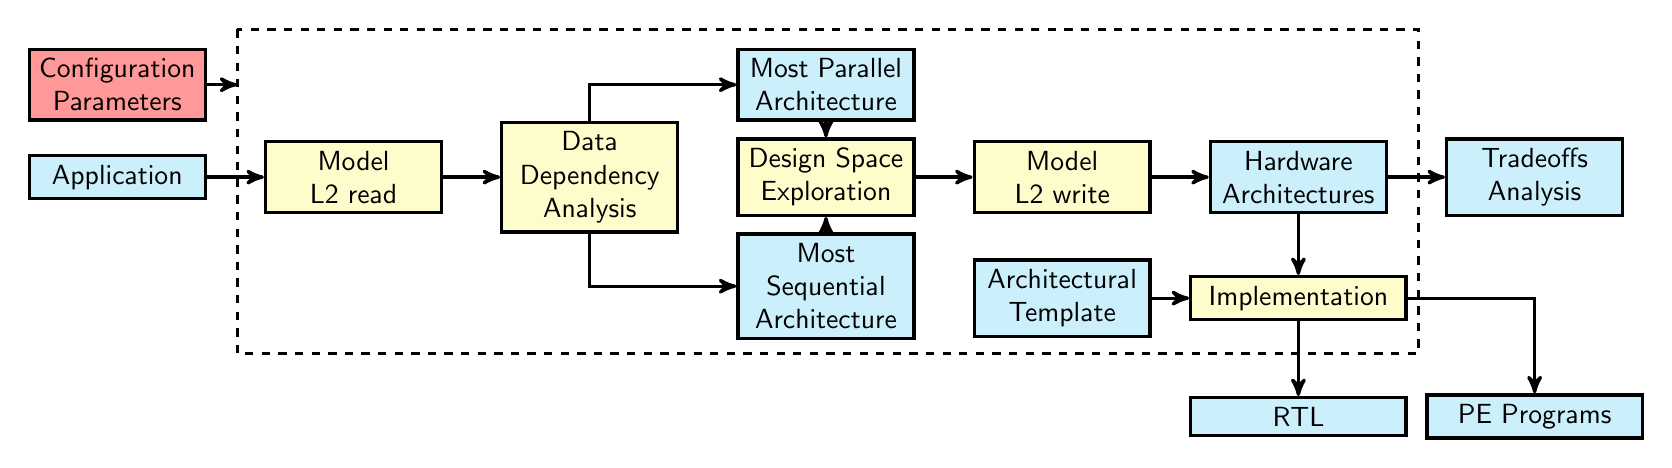
\begin{tikzpicture}[
    bus/.style={rectangle,thick,draw,anchor=north,
		minimum width=1.5cm,minimum height = 0.5mm},
    archb/.style={rectangle,thick,draw,fill=blue!60,anchor=north,
		minimum width=0.2cm},
    archm/.style={rectangle,thick,draw,fill=magenta!60,anchor=north,
		minimum width=0.2cm},
    select/.style={circle,thick,draw,anchor=north,
		minimum width=0.4cm},
% Event style
    event/.style={rectangle,very thick,draw,fill=yellow!20,text width=2cm,
		text centered,font=\sffamily,anchor=north},
%  For compatability with PGF CVS add the absolute option:
   absolute
    ]
   \begin{scope}[xshift=-7.5cm,yshift=-5cm,very thick,
		node distance=3cm,on grid,>=stealth',
		block/.style={rectangle,draw,font=\sffamily,fill=cyan!20,text width=2cm,text centered}]

    % Place nodes
    \node [block] (app) {Application};
    %\node [] (start_dash) [below=of app.west, below=80pt,xshift=-10pt]{};
    %\node [] (end_dash) [below=of app.east, below=80pt]{};
    %\node [] (dash label) [right=of end_dash, right=2pt]{Manual};

    %\node [] (start_solid_dash) [below=of start_dash, below=10pt]{};
    %\node [] (end_solid_dash) [below=of end_dash, below=10pt]{};
    %\node [] (dash label) [right=of end_solid_dash, right=2pt]{Automated};

    \node [event,right=of app] (l21){Model L2 read};
    \node [event,right=of l21] (ddg_ana){Data Dependency Analysis};

    \node [event, right of=ddg_ana] (dse) {Design Space Exploration};
    \node [block, above=of dse,above=20 pt] (dfg_full) {Most Parallel Architecture};
    \node [block, below=of dse,below=20pt] (dfg_seq) {Most Sequential Architecture};
%    \node [circle,draw,fill=blue!100,right=of dse,text=white,font=\sffamily] (l22){2};
    \node [event,right=of dse] (l22){Model L2 write};

    \node [block, right of=l22] (dse_analysis) {Hardware Architectures};
    \node [block, right of=dse_analysis] (tradeoff) {Tradeoffs Analysis};
  \node [event , below of=dse_analysis, below = -50pt, text width=2.5cm] (impl) {Implementation};
  \node [block, below of=impl, below = -50pt, text width=2.5cm] (rtl) {RTL};
  \node [block, right of=rtl, text width=2.5cm] (fu_prog) {PE Programs};
      \node [block, left of=impl] (temp_arch) {Architectural\\Template};
    \node [block, fill=red!40,above=of app,above = 20pt] (params) {Configuration Parameters};

    \coordinate [right of= params, xshift=-42pt, above = 20pt] (top_left_box);
    \coordinate [right of= impl, xshift=-42pt, below = 20pt] (bottom_right_box);
    \coordinate [right of= params, xshift=-42pt] (param_anchor);
    \draw [dashed] (top_left_box) rectangle (bottom_right_box);

    %\node [block, right of=dfg_seq] (dfg_seq_analysis) {Analysis};

    % Draw edges
%    \draw [->] (app) -- ( ddg_ana);
    \draw [->] (app) -- ( l21);
    \draw [->] (l21) -- ( ddg_ana);
    \draw [->] (ddg_ana) |- (dfg_full);
    \draw [->] (ddg_ana) |- (dfg_seq);
    \draw [->] (dfg_full) -- (dse);
    \draw [->] (dfg_seq) -- (dse);
%    \draw [->] (dse) -- (dse_analysis);
    \draw [->] (dse) -- (l22);
    \draw [->] (l22) -- (dse_analysis);
    \draw [->] (dse_analysis) -- (impl);
    \draw [->] (dse_analysis) -- (tradeoff);
   \draw [->] (temp_arch) -- (impl);
 \draw [->] (impl) -- (rtl);
 \draw [->] (impl) -| (fu_prog);
 %\draw [-, dashed] (start_dash.west) -- (end_dash.east);
 %\draw [-] (start_solid_dash.west) -- (end_solid_dash.east);

    \draw [->] (params) -- (param_anchor);

\end{scope}
\end{tikzpicture}
\end{document}
